\section{Фотометрическая декомпозиция}
На данном этапе производится детальный анализ изображений видимых с ребра галактик в полосе Stripe 82, с целью оценки вертикальных и радиальных масштабов их звездных дисков.

Для описания распределения яркости вдоль направления малой оси галактики, видимой с ребра, обычно применяется модель самогравитирующего изотермического слоя \cite{1981A&A....95..105V}, для которого \ref{eq:sech}:
\begin{equation}
I(z) = I_0\sech^2(z/z_0)
\label{eq:sech}
\end{equation}
где $z_0$ -- вертикальный масштаб, то есть масштаб распределения яркости вдоль перпендикулярного к плоскости диска направления (вдоль координаты z). В рамках этой модели вертикальный масштаб связан с вертикальной
дисперсией скоростей звезд и их объемной и поверхностной плотностью. 
Вблизи от плоскости галактики $(z/z_0 \ll 1)$: $\sech^2(z/z_0) = exp(-z^2/z_0^2)$.
Вдали от плоскости $(z/z_0 \gg 1)$: $\sech^2(z/z_0) = 4exp(-2z/z_0^2) $.
Можно ввести еще одну формулу \ref{eq:exp} экспоненциального закона, совпадающую с \ref{eq:sech} в случаях $z/z_0 \ll 1$ и $z/z_0 \gg 1$:
\begin{equation}
    I(z) = exp(-|z|/h_z),
    \label{eq:exp}
\end{equation}
где $h_z$ -- экспоненциальный масштаб распределения яркости вдоль перпендикулярного к диску направления (вдоль координаты z). Формулы \ref{eq:sech} и \ref{eq:exp} связаны через соотношение $z_0 = 2h_z$.
Наблюдения показывают, что для некоторых галактик формула \ref{eq:exp} вполне адекватно описывает наблюдаемое распределение яркости. 

В свою очередь, распределение яркости в радиальном направлении в диске спиральной галактики, видимой плашмя, может быть хорошо описано экспоненциальным законом с радиальным масштабом $h_r$ \cite{1959HDP....53..275D} \cite{1940BHarO.914....9P}:
\begin{equation}
    I(r) = I_0exp(-r/h_r)
    \label{eq:radexp}
\end{equation}
Таким образом, $h_z$ и $h_r$ – вертикальный и радиальный экспоненциальные масштабы диска. Они могут быть использованы для описания глобальной фотометрической структуры галактик. В данном разделе получение и анализ этих параметров является основной задачей. 

Мы можем совместить формулы распределения поверхностной яркости в радиальном и вертикальном направлениях. Модель диска спиральной галактики в этом случае будет выражаться следующей формулой:
\begin{equation}
    I(r,z) = I_0e^{-r/h}sech^2{z/z_0}
    \label{eq: combined}
\end{equation}
Здесь радиальный масштаб обозначается как \textit{h}, а вертикальный – как $z_0$. Такие обозначения будут применены и для следующих формул данного раздела.
В работе van der Kruit P.C., Searle L. \cite{1981A&A....95..105V} вычислена поверхностная яркость с законом распределения \ref{eq: combined} для спиральной галактики, наблюдаемой с ребра:
\begin{equation}
    \mu(r,z) = \mu(0,0)(r/h)K_1(r/h)sech^2(z/z_0)
    \label{vanderkruit}
\end{equation}
где $K_1$ -- модифицированная функция Бесселя первого порядка. Центральная поверхностная яркость выражается следующим образом:
\begin{equation}
    \mu(0,0) = 2hL_0,
\end{equation}
где $L_0$ -- центральная поверхностная яркость.
Позднее в работе того же автора \cite{1988A&A...192..117V} было предложено использовать более общий закон для описания распределения плотности светящегося вещества в галактике вдоль координаты z:
\begin{equation}
    \rho(z) = 2^{-2/n}\rho_0\sech^{2/n}(nz/(2z_0))\hspace{2em}(n>0), 
    \label{eq:new_law}
\end{equation}
в котором степень $2/n$ регулирует форму распределения.
при $n = 1$ формула \ref{eq:new_law} переходит в модель изотермического слоя (формула \ref{eq:sech}), при $n = \infty$ в экспоненциальный закон (формула \ref{eq:exp}).
Отсюда, согласно \cite{1988A&A...192..117V}, получается следующая формула распределения поверхностной яркости для видимой с ребра галактики:
\begin{equation}
    I(r,z) = \mu(0,0)(r/h)K_1(r/h)sech^{2/n}(nz/(2z_0))
    \label{eq:final_law}
\end{equation}

Важно отметить, что в процессе выполнения фотометрической декомпозиции был зафиксирован параметр $n$, он был принят равным значению $n = 100$. Тогда, согласно формуле \ref{eq:final_law}, $\sech^{2/n}(nz/(2z_0)) \approx exp(z/z_0)$. То есть распределение яркости всех галактик вдоль вертикального направления было аппроксимировано простым экспоненциальным законом.

Для получения начального приближения вертикального и радиального масштабов диска была выполнена одномерная фотометрическая декомпозиция компонент диска и балджа. Для этого были модифицированы python скрипты, подготовленные научным руководителем, Савченко С.С. \footnote{https://bitbucket.org/latrop/decomposer/src/master/}. Используя результаты одномерной декомпозиции в качестве входных параметров была осуществлена двумерная декомпозиция.
Порядок выполнения фотометрической декомпозиции был следующий:
\begin{enumerate}
    \item Изначально была составлена "золотая"$\,$         выборка галактик, наблюдаемых точно с ребра. Это определялось, например, по расположению пылевой полосы. Также критериями отбора галактик являлось наличие регулярной структуры без особенностей, отсутствие ярких источников в близкой окрестности галактики (чтобы само тело галактики не сильно перекрывалось другими источниками и не было ярких звёзд поблизости). Полученная выборка включает 73 объекта.
    \item Перед выполнением одномерной декомпозиции были заранее подготовлены обрезанные изображения галактик (со стороной изображения 3 размера большой полуоси по горизонтали, и малой оси по вертикали), соразмерные файлы масок, файлы весов, файлы psf, помогающие учитывать влияние оптической системы и атмосферной турбулентности.
    \item Для выполнения декомпозиции достаточно указать номер галактики в выборке в качестве ключа при запуске скрипта. В процессе работы программы для каждой галактики было построено 2 модели: первая -- простая модель, использующая функцию \ref{eq:final_law} (соответсвующая функция в Imfit -- EdgeOnDisk) и описывающая галактику как объект, расположенный точно с ребра. Во второй модели добавляется компонента балджа, аппроксимируемая функцией Серсика:
    \begin{equation}
        I(a) = I_eexp\Bigg\{-b_n\Bigg[\bigg(\frac{a}{r_e}^{1/n}-1\bigg)\Bigg]\Bigg\},
        \label{Sersic}
    \end{equation}
    где $I_e$ -- поверхностная яркость на эффективном радиусе $r_e$,  n -- индекс Серсика, значение параметра $b_n$ формально задает решение трансцендентного выражения $\Gamma(2n) = 2\gamma(2n, b_n)$. Здесь $\Gamma(a)$ -- гамма-функция, а $\gamma(a,x)$ -- неполная гамма-функция. 
    \item Для каждой из двух моделей было автоматически посчитано значение BIC (the Bayesian information criterion), расчитываемое по формуле: $BIC = -2\ln\textit{L} + k\ln(n)$, где \textit{L} -- максимальное значение функции правдоподобия наблюдаемой выборки с известным числом параметров, k -- количество свободных параметров, n -- количество незамаскрированных пикселей на изображении. Выбиралась та модель, значение BIC для которой наименьшее. 
    \item На выходе мы имеем конфиругационный файл Imfit, в котором описаны 7 параметров диска: 
    
    \begin{tabular}{p{40mm}p{5mm}p{90mm}}
    
    \texttt{X0} & -- & координата центра по оси X изображения  \\
    \texttt{Y0} & -- & координата центра по оси X изображения \\
    \texttt{EdgeOnDisk} & -- &функция для аппроксимации \\
    \texttt{PA} & -- &позиционный угол (угол между осью Y изображения и осью координаты r, отсчитываемый против часовой стрелки  \\
    \texttt{$L\_0$} & -- &центральная плотность светимости $L_0$ \\
    \texttt{h} & -- & радиальный масштаб $h$ \\
    \texttt{n} & -- & индекс Серсика $n$ \\
    \texttt{$z\_0$} & -- & вертикальный масштаб $z_0$
    \end{tabular}

    \item Следующий выполненный этап -- двумерная декомпозиция в Imfit\cite{2015ApJ...799..226E}. На вход программы осуществлялась подача изображения галактики, конфигурационного файла с комбинацией двумерных функций (результат одномерной декомпозиции), которые должны аппроксимировать распределение поверхностной яркости при декомпозиции, также файлы с маской и весами, psf-изображение.
    \item Построены модельные изображения галактик, описываемых комбинацией двумерных функций с заданными параметрами.
    \item Получены разностные изображения и вычислена статистическая разница реального и модельного изображений галактики (по критерию $\chi^2$ ) c применением информации о достоверности значений
в пикселях, содержащейся в изображениях масок и весов.
    \item Выполнена корректировка параметров модельных двумерных функций в сторону уменьшения статистической разницы $\chi^2$ методом градиентного спуска.
    \item Построены срезы вдоль большой и малой полуоси галактики в сравнении с моделями, описываемыми полученными в процессе двумерной декомпозиции параметрами (Рис. \ref{fig:slices}). Получены изображения моделей и их разностей с изображениями реальных галактик (Рис. \ref{fig:models}).
    
\end{enumerate}

\begin{figure}[p]
    \centering
    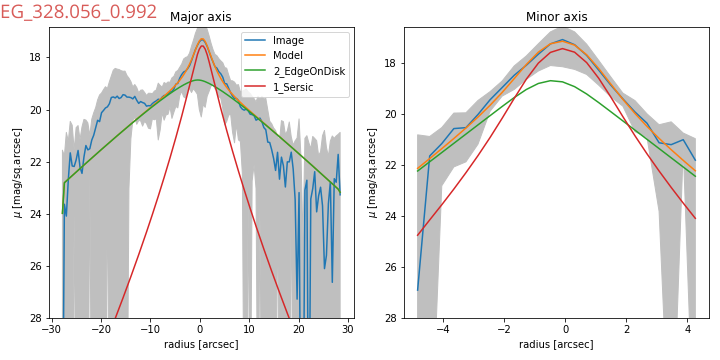
\includegraphics[width=.9\textwidth]{plot_results/4.png}\hfill\\
    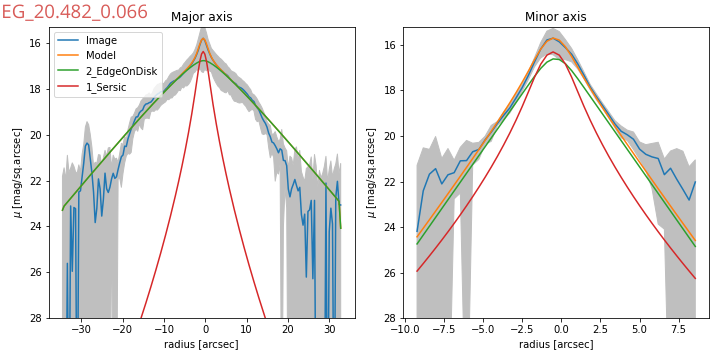
\includegraphics[width=.9\textwidth]{plot_results/6.png}\hfill\\
    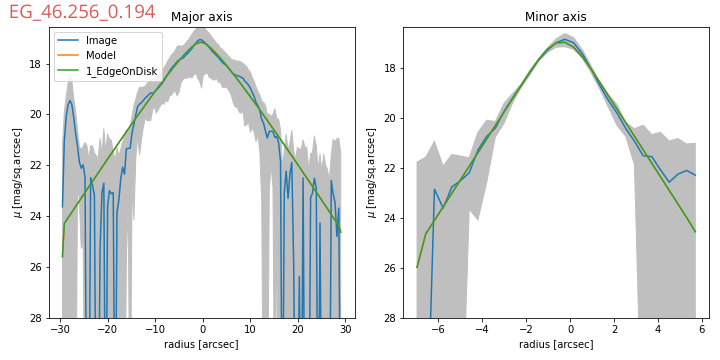
\includegraphics[width=.9\textwidth]{plot_results/5.png}\hfill\\

    \caption{Примеры полученных результатов двумерной декомпозиции: левая панель -- разрез вдоль большой полуоси галактики, правая панель -- разрез вдоль малой полуоси галактики. Зеленым цветом изображена модельная компонента диска, красным -- компонента балджа (если имеется), желтым -- сумма двух компонент. }\label{fig:slices}
\end{figure}

\begin{figure}[p]
    \centering
    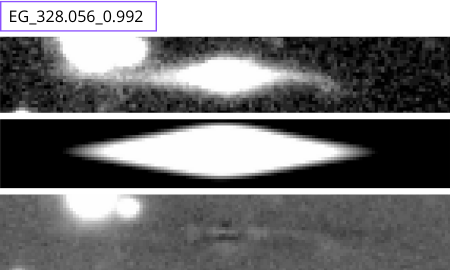
\includegraphics[width=.7\textwidth]{plot_results/1.png}\hfill\\
    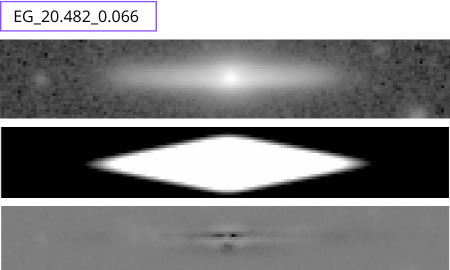
\includegraphics[width=.7\textwidth]{plot_results/2.png}\hfill\\
    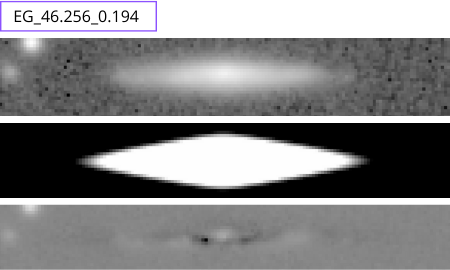
\includegraphics[width=.7\textwidth]{plot_results/3.png}\hfill\\

    \caption{Примеры полученных результатов двумерной декомпозиции: левая панель -- изображение реальной галактики, средняя панель -- модель, правая панель -- разность изображения реальной галактики и модели.  }\label{fig:models}
\end{figure}